\documentclass[]{book}
\usepackage{lmodern}
\usepackage{amssymb,amsmath}
\usepackage{ifxetex,ifluatex}
\usepackage{fixltx2e} % provides \textsubscript
\ifnum 0\ifxetex 1\fi\ifluatex 1\fi=0 % if pdftex
  \usepackage[T1]{fontenc}
  \usepackage[utf8]{inputenc}
\else % if luatex or xelatex
  \ifxetex
    \usepackage{mathspec}
  \else
    \usepackage{fontspec}
  \fi
  \defaultfontfeatures{Ligatures=TeX,Scale=MatchLowercase}
\fi
% use upquote if available, for straight quotes in verbatim environments
\IfFileExists{upquote.sty}{\usepackage{upquote}}{}
% use microtype if available
\IfFileExists{microtype.sty}{%
\usepackage{microtype}
\UseMicrotypeSet[protrusion]{basicmath} % disable protrusion for tt fonts
}{}
\usepackage{hyperref}
\hypersetup{unicode=true,
            pdftitle={This is us: making CSAFE stronger each week},
            pdfauthor={CSAFE},
            pdfborder={0 0 0},
            breaklinks=true}
\urlstyle{same}  % don't use monospace font for urls
\usepackage{natbib}
\bibliographystyle{apalike}
\usepackage{color}
\usepackage{fancyvrb}
\newcommand{\VerbBar}{|}
\newcommand{\VERB}{\Verb[commandchars=\\\{\}]}
\DefineVerbatimEnvironment{Highlighting}{Verbatim}{commandchars=\\\{\}}
% Add ',fontsize=\small' for more characters per line
\usepackage{framed}
\definecolor{shadecolor}{RGB}{248,248,248}
\newenvironment{Shaded}{\begin{snugshade}}{\end{snugshade}}
\newcommand{\AlertTok}[1]{\textcolor[rgb]{0.94,0.16,0.16}{#1}}
\newcommand{\AnnotationTok}[1]{\textcolor[rgb]{0.56,0.35,0.01}{\textbf{\textit{#1}}}}
\newcommand{\AttributeTok}[1]{\textcolor[rgb]{0.77,0.63,0.00}{#1}}
\newcommand{\BaseNTok}[1]{\textcolor[rgb]{0.00,0.00,0.81}{#1}}
\newcommand{\BuiltInTok}[1]{#1}
\newcommand{\CharTok}[1]{\textcolor[rgb]{0.31,0.60,0.02}{#1}}
\newcommand{\CommentTok}[1]{\textcolor[rgb]{0.56,0.35,0.01}{\textit{#1}}}
\newcommand{\CommentVarTok}[1]{\textcolor[rgb]{0.56,0.35,0.01}{\textbf{\textit{#1}}}}
\newcommand{\ConstantTok}[1]{\textcolor[rgb]{0.00,0.00,0.00}{#1}}
\newcommand{\ControlFlowTok}[1]{\textcolor[rgb]{0.13,0.29,0.53}{\textbf{#1}}}
\newcommand{\DataTypeTok}[1]{\textcolor[rgb]{0.13,0.29,0.53}{#1}}
\newcommand{\DecValTok}[1]{\textcolor[rgb]{0.00,0.00,0.81}{#1}}
\newcommand{\DocumentationTok}[1]{\textcolor[rgb]{0.56,0.35,0.01}{\textbf{\textit{#1}}}}
\newcommand{\ErrorTok}[1]{\textcolor[rgb]{0.64,0.00,0.00}{\textbf{#1}}}
\newcommand{\ExtensionTok}[1]{#1}
\newcommand{\FloatTok}[1]{\textcolor[rgb]{0.00,0.00,0.81}{#1}}
\newcommand{\FunctionTok}[1]{\textcolor[rgb]{0.00,0.00,0.00}{#1}}
\newcommand{\ImportTok}[1]{#1}
\newcommand{\InformationTok}[1]{\textcolor[rgb]{0.56,0.35,0.01}{\textbf{\textit{#1}}}}
\newcommand{\KeywordTok}[1]{\textcolor[rgb]{0.13,0.29,0.53}{\textbf{#1}}}
\newcommand{\NormalTok}[1]{#1}
\newcommand{\OperatorTok}[1]{\textcolor[rgb]{0.81,0.36,0.00}{\textbf{#1}}}
\newcommand{\OtherTok}[1]{\textcolor[rgb]{0.56,0.35,0.01}{#1}}
\newcommand{\PreprocessorTok}[1]{\textcolor[rgb]{0.56,0.35,0.01}{\textit{#1}}}
\newcommand{\RegionMarkerTok}[1]{#1}
\newcommand{\SpecialCharTok}[1]{\textcolor[rgb]{0.00,0.00,0.00}{#1}}
\newcommand{\SpecialStringTok}[1]{\textcolor[rgb]{0.31,0.60,0.02}{#1}}
\newcommand{\StringTok}[1]{\textcolor[rgb]{0.31,0.60,0.02}{#1}}
\newcommand{\VariableTok}[1]{\textcolor[rgb]{0.00,0.00,0.00}{#1}}
\newcommand{\VerbatimStringTok}[1]{\textcolor[rgb]{0.31,0.60,0.02}{#1}}
\newcommand{\WarningTok}[1]{\textcolor[rgb]{0.56,0.35,0.01}{\textbf{\textit{#1}}}}
\usepackage{longtable,booktabs}
\usepackage{graphicx,grffile}
\makeatletter
\def\maxwidth{\ifdim\Gin@nat@width>\linewidth\linewidth\else\Gin@nat@width\fi}
\def\maxheight{\ifdim\Gin@nat@height>\textheight\textheight\else\Gin@nat@height\fi}
\makeatother
% Scale images if necessary, so that they will not overflow the page
% margins by default, and it is still possible to overwrite the defaults
% using explicit options in \includegraphics[width, height, ...]{}
\setkeys{Gin}{width=\maxwidth,height=\maxheight,keepaspectratio}
\IfFileExists{parskip.sty}{%
\usepackage{parskip}
}{% else
\setlength{\parindent}{0pt}
\setlength{\parskip}{6pt plus 2pt minus 1pt}
}
\setlength{\emergencystretch}{3em}  % prevent overfull lines
\providecommand{\tightlist}{%
  \setlength{\itemsep}{0pt}\setlength{\parskip}{0pt}}
\setcounter{secnumdepth}{5}
% Redefines (sub)paragraphs to behave more like sections
\ifx\paragraph\undefined\else
\let\oldparagraph\paragraph
\renewcommand{\paragraph}[1]{\oldparagraph{#1}\mbox{}}
\fi
\ifx\subparagraph\undefined\else
\let\oldsubparagraph\subparagraph
\renewcommand{\subparagraph}[1]{\oldsubparagraph{#1}\mbox{}}
\fi

%%% Use protect on footnotes to avoid problems with footnotes in titles
\let\rmarkdownfootnote\footnote%
\def\footnote{\protect\rmarkdownfootnote}

%%% Change title format to be more compact
\usepackage{titling}

% Create subtitle command for use in maketitle
\providecommand{\subtitle}[1]{
  \posttitle{
    \begin{center}\large#1\end{center}
    }
}

\setlength{\droptitle}{-2em}

  \title{This is us: making CSAFE stronger each week}
    \pretitle{\vspace{\droptitle}\centering\huge}
  \posttitle{\par}
    \author{CSAFE}
    \preauthor{\centering\large\emph}
  \postauthor{\par}
      \predate{\centering\large\emph}
  \postdate{\par}
    \date{2019-09-05}

\usepackage{booktabs}
\usepackage{amsthm}
\makeatletter
\def\thm@space@setup{%
  \thm@preskip=8pt plus 2pt minus 4pt
  \thm@postskip=\thm@preskip
}
\makeatother

\begin{document}
\maketitle

{
\setcounter{tocdepth}{1}
\tableofcontents
}
\hypertarget{prerequisites}{%
\chapter{Prerequisites}\label{prerequisites}}

This is a \emph{sample} book written in \textbf{Markdown}. You can use anything that Pandoc's Markdown supports, e.g., a math equation \(a^2 + b^2 = c^2\).

The \textbf{bookdown} package can be installed from CRAN or Github:

\begin{Shaded}
\begin{Highlighting}[]
\KeywordTok{install.packages}\NormalTok{(}\StringTok{"bookdown"}\NormalTok{)}
\CommentTok{# or the development version}
\CommentTok{# devtools::install_github("rstudio/bookdown")}
\end{Highlighting}
\end{Shaded}

Remember each Rmd file contains one and only one chapter, and a chapter is defined by the first-level heading \texttt{\#}.

To compile this example to PDF, you need XeLaTeX. You are recommended to install TinyTeX (which includes XeLaTeX): \url{https://yihui.name/tinytex/}.

\hypertarget{intro}{%
\chapter{Introduction}\label{intro}}

This section will become the section for the administrative updates/organization once we have figured out how to use all of the bookdown features for our purposes.

You can label chapter and section titles using \texttt{\{\#label\}} after them, e.g., we can reference Chapter \ref{intro}. If you do not manually label them, there will be automatic labels anyway, e.g., Chapter \ref{glass}.

Figures and tables with captions will be placed in \texttt{figure} and \texttt{table} environments, respectively.

\begin{Shaded}
\begin{Highlighting}[]
\KeywordTok{par}\NormalTok{(}\DataTypeTok{mar =} \KeywordTok{c}\NormalTok{(}\DecValTok{4}\NormalTok{, }\DecValTok{4}\NormalTok{, }\FloatTok{.1}\NormalTok{, }\FloatTok{.1}\NormalTok{))}
\KeywordTok{plot}\NormalTok{(pressure, }\DataTypeTok{type =} \StringTok{'b'}\NormalTok{, }\DataTypeTok{pch =} \DecValTok{19}\NormalTok{)}
\end{Highlighting}
\end{Shaded}

\begin{figure}

{\centering 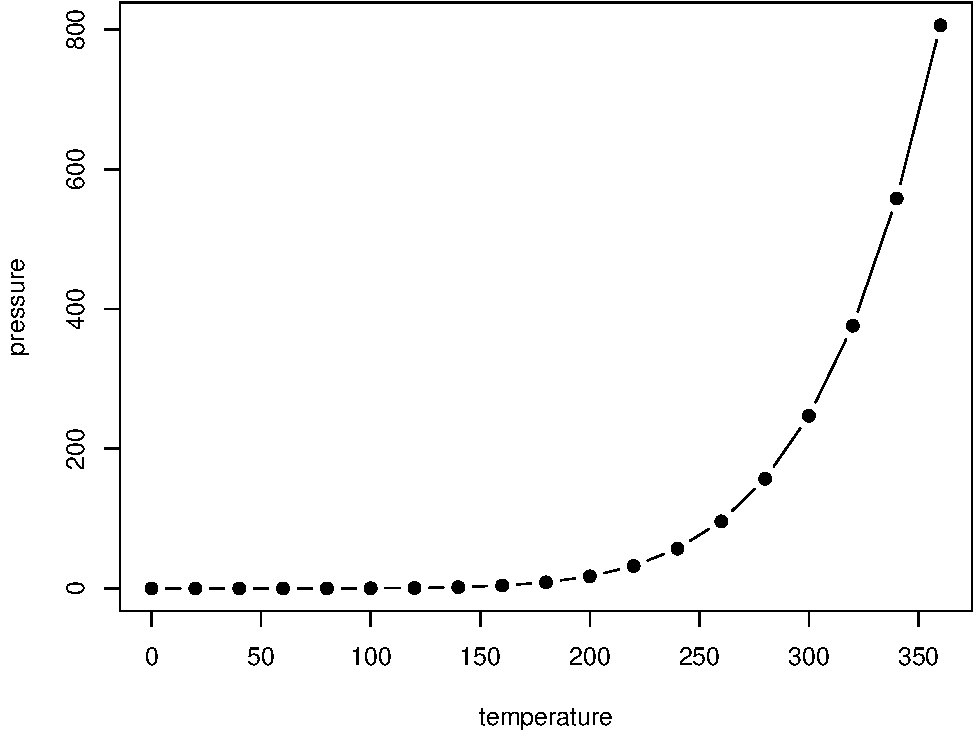
\includegraphics[width=0.8\linewidth]{bookdown-demo_files/figure-latex/nice-fig-1} 

}

\caption{Here is a nice figure!}\label{fig:nice-fig}
\end{figure}

Reference a figure by its code chunk label with the \texttt{fig:} prefix, e.g., see Figure \ref{fig:nice-fig}. Similarly, you can reference tables generated from \texttt{knitr::kable()}, e.g., see Table \ref{tab:nice-tab}.

\begin{Shaded}
\begin{Highlighting}[]
\NormalTok{knitr}\OperatorTok{::}\KeywordTok{kable}\NormalTok{(}
  \KeywordTok{head}\NormalTok{(iris, }\DecValTok{20}\NormalTok{), }\DataTypeTok{caption =} \StringTok{'Here is a nice table!'}\NormalTok{,}
  \DataTypeTok{booktabs =} \OtherTok{TRUE}
\NormalTok{)}
\end{Highlighting}
\end{Shaded}

\begin{table}[t]

\caption{\label{tab:nice-tab}Here is a nice table!}
\centering
\begin{tabular}{rrrrl}
\toprule
Sepal.Length & Sepal.Width & Petal.Length & Petal.Width & Species\\
\midrule
5.1 & 3.5 & 1.4 & 0.2 & setosa\\
4.9 & 3.0 & 1.4 & 0.2 & setosa\\
4.7 & 3.2 & 1.3 & 0.2 & setosa\\
4.6 & 3.1 & 1.5 & 0.2 & setosa\\
5.0 & 3.6 & 1.4 & 0.2 & setosa\\
\addlinespace
5.4 & 3.9 & 1.7 & 0.4 & setosa\\
4.6 & 3.4 & 1.4 & 0.3 & setosa\\
5.0 & 3.4 & 1.5 & 0.2 & setosa\\
4.4 & 2.9 & 1.4 & 0.2 & setosa\\
4.9 & 3.1 & 1.5 & 0.1 & setosa\\
\addlinespace
5.4 & 3.7 & 1.5 & 0.2 & setosa\\
4.8 & 3.4 & 1.6 & 0.2 & setosa\\
4.8 & 3.0 & 1.4 & 0.1 & setosa\\
4.3 & 3.0 & 1.1 & 0.1 & setosa\\
5.8 & 4.0 & 1.2 & 0.2 & setosa\\
\addlinespace
5.7 & 4.4 & 1.5 & 0.4 & setosa\\
5.4 & 3.9 & 1.3 & 0.4 & setosa\\
5.1 & 3.5 & 1.4 & 0.3 & setosa\\
5.7 & 3.8 & 1.7 & 0.3 & setosa\\
5.1 & 3.8 & 1.5 & 0.3 & setosa\\
\bottomrule
\end{tabular}
\end{table}

You can write citations, too. For example, we are using the \textbf{bookdown} package \citep{R-bookdown} in this sample book, which was built on top of R Markdown and \textbf{knitr} \citep{xie2015}.

\hypertarget{bullets}{%
\chapter{Project CC: Bullets and Cartridge Cases}\label{bullets}}

For both bullets and cartridge cases we are dealing with several inter-related aspects, that we want to address independently.

Those are:

\begin{enumerate}
\def\labelenumi{\arabic{enumi}.}
\item
  data collection
\item
  computational tools
\item
  similarity scores

  \begin{enumerate}
  \def\labelenumii{\arabic{enumii}.}
  \item
    for bullet lands:

    \begin{enumerate}
    \def\labelenumiii{\alph{enumiii}.}
    \tightlist
    \item
      crosscut identification
    \item
      groove location
    \item
      curvature removal
    \item
      alignment of signatures
    \item
      feature extraction
    \item
      matching with trained Random Forest
    \end{enumerate}
  \item
    for breech faces
  \end{enumerate}
\item
  analysis of results
\item
  communication of results and methods
\end{enumerate}

\hypertarget{data-collection}{%
\section{Data Collection}\label{data-collection}}

\hypertarget{lapd}{%
\subsection{LAPD}\label{lapd}}

All bullets are collected by Srinivasan Rathinam, LAPD.

\hypertarget{main-study}{%
\subsubsection{Main study}\label{main-study}}

4 bullets per barrel for 626 Beretta 92 F/FS firearms , ammunition used are 9 mm Luger Winchester 115 grain with a Copper surface.

scans are on Raven.

evaluation: Yawei is going to work through all 626 barrels of knowns to assess similarity scores

\begin{figure}

{\centering 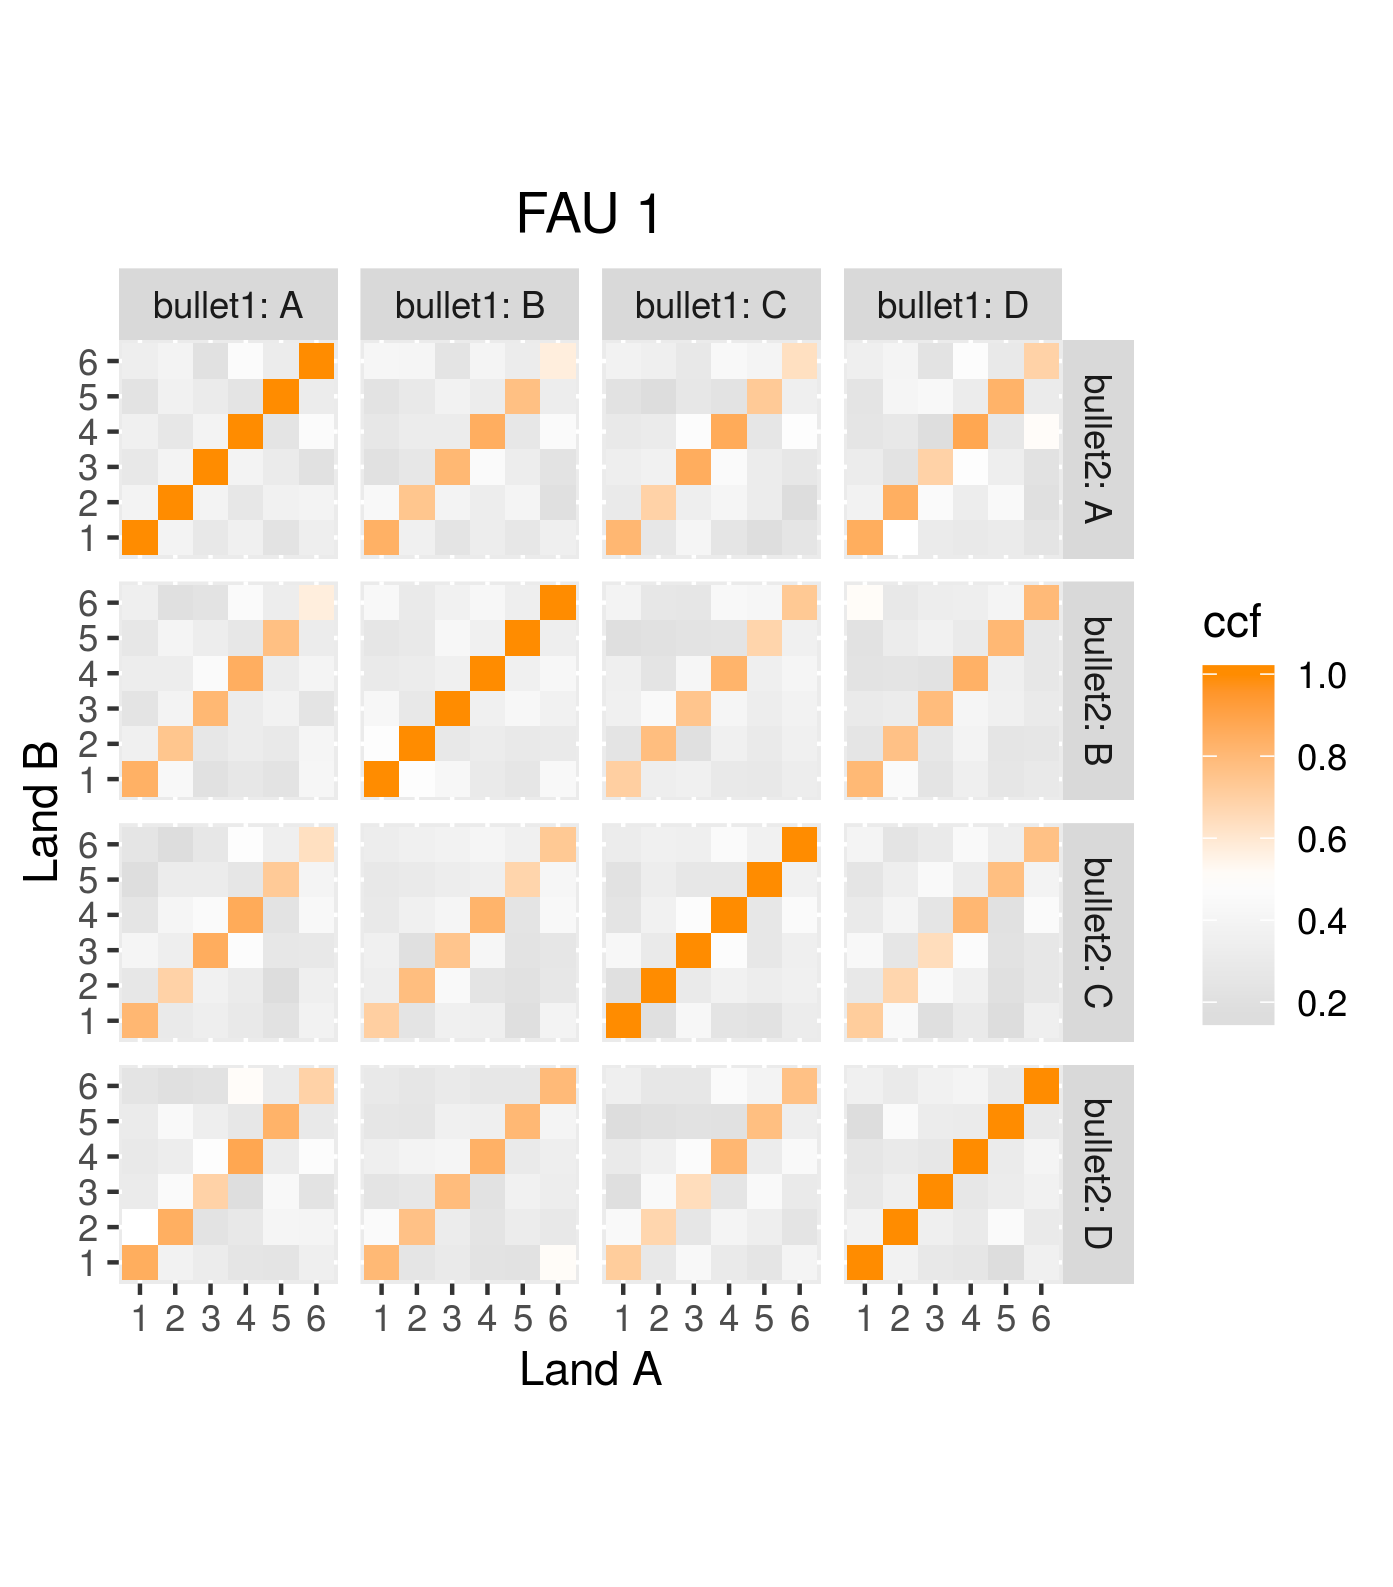
\includegraphics[width=0.5\linewidth]{images/yawei/results-FAU-1} 

}

\caption{Results from assessing scans of barrel FAU 1 similarity.}\label{fig:unnamed-chunk-3}
\end{figure}

\begin{figure}

{\centering 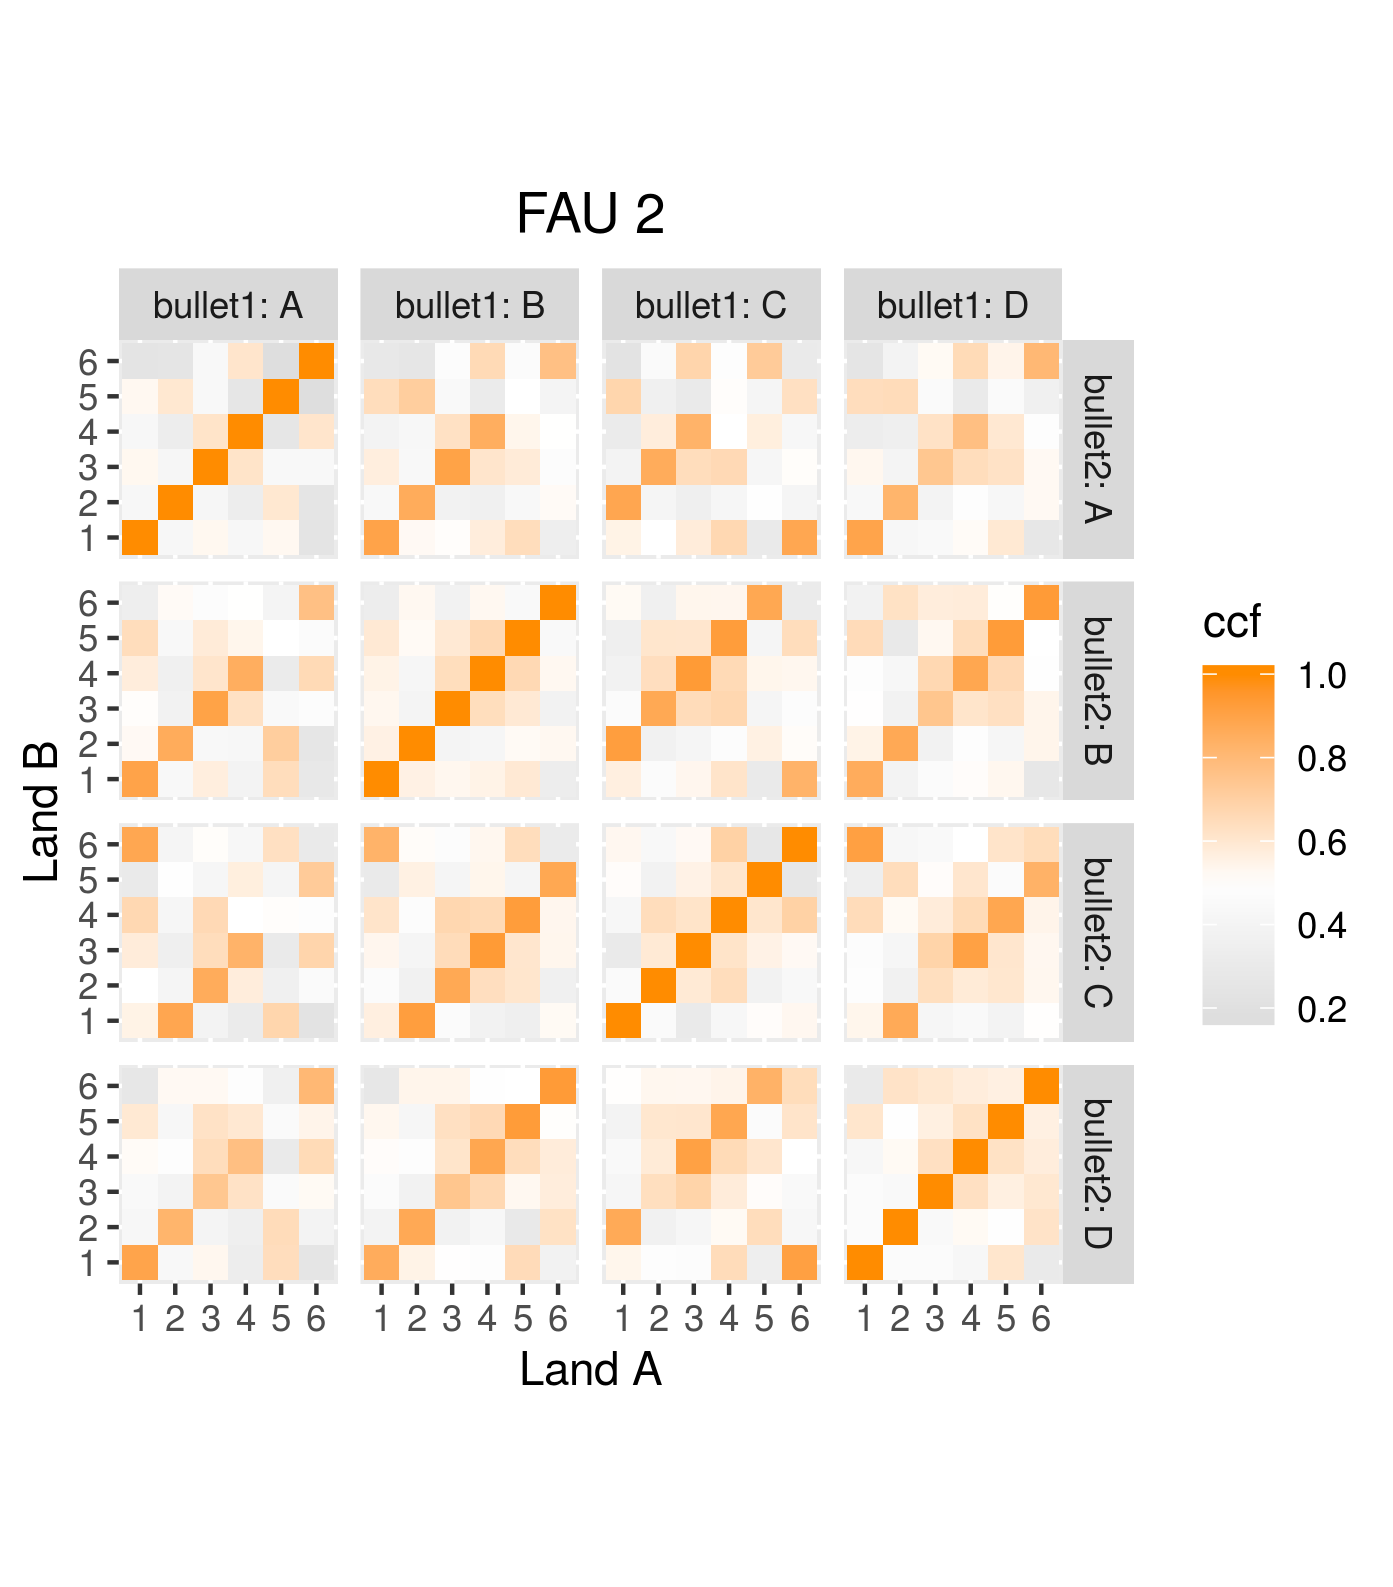
\includegraphics[width=0.5\linewidth]{images/yawei/results-FAU-2} 

}

\caption{Results from assessing scans of barrel FAU 2 similarity.}\label{fig:unnamed-chunk-4}
\end{figure}

\hypertarget{follow-up-study}{%
\subsubsection{follow-up study}\label{follow-up-study}}

4 bullets per barrel for 96 of the original 626 Beretta firearms using different ammunition

bullets are being scanned

\hypertarget{hamby-sets}{%
\subsection{Hamby Sets}\label{hamby-sets}}

Scans for Hamby Sets 10, 36, 44, and 224

Scans for 3 replicates of clones for Hamby 224

\hypertarget{houston-tests}{%
\subsection{Houston Tests}\label{houston-tests}}

contact: Melissa Nally, Houston FSI

\hypertarget{pre-study}{%
\subsubsection{Pre-study}\label{pre-study}}

3 kits with 23 bullets each

\begin{figure}

{\centering 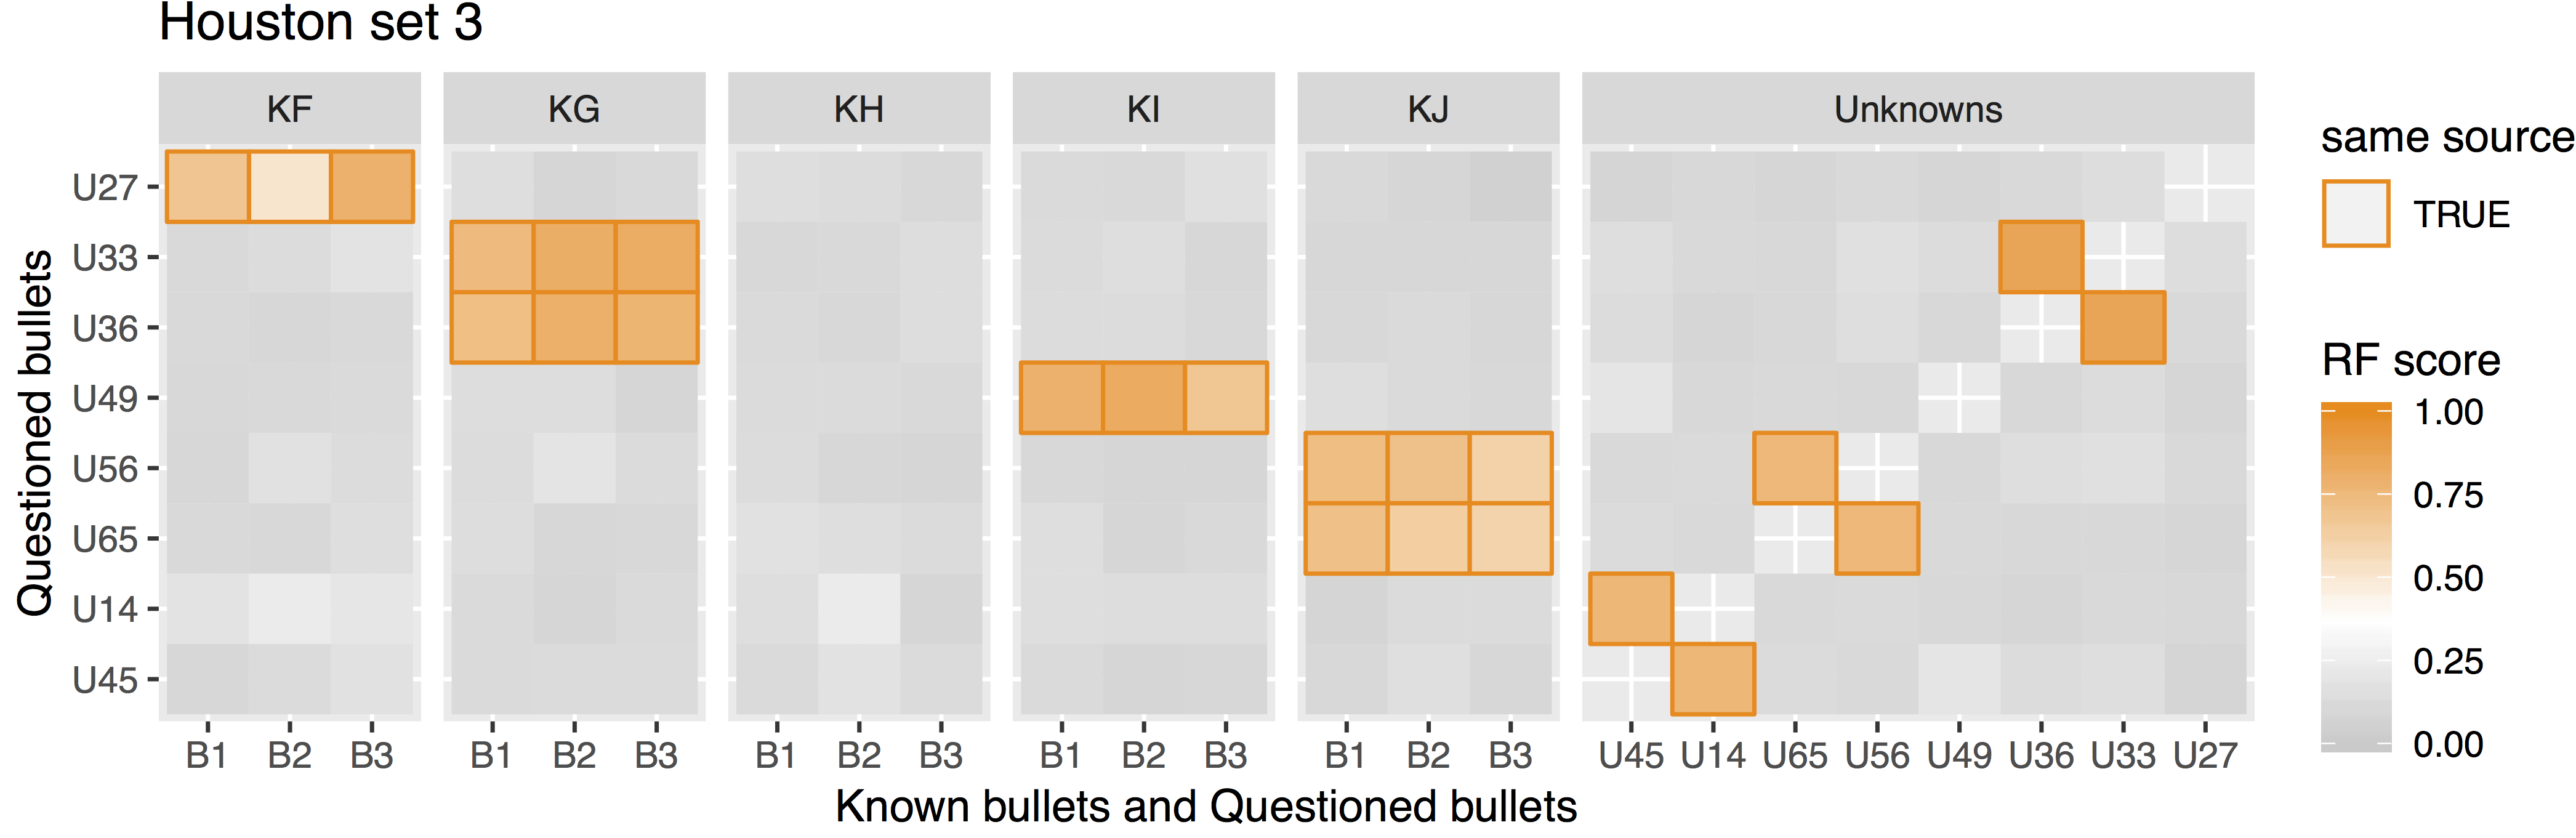
\includegraphics[width=58.11in]{images/heike/houston-pre-set3} 

}

\caption{Bullet-to-bullet similarity scores for questioned bullets (y-axis) compared to all other bullets of the test set (x-axis).}\label{fig:unnamed-chunk-5}
\end{figure}

evaluation included in submission to JFI

\hypertarget{study}{%
\subsubsection{Study}\label{study}}

4 kits with 20 bullets each

scans done, evaluation finished, some scans of doubtful quality

\hypertarget{houston-persistence}{%
\subsection{Houston Persistence}\label{houston-persistence}}

contact: Melissa Nally, Houston FSI

8 barrels with 40 fired bullets each

\hypertarget{st-louis-persistence}{%
\subsection{St Louis persistence}\label{st-louis-persistence}}

contact: Steve Kramer, St Louis PD

2 barrels with 192 fired bullets each (2 bullets collected every 25 shots)

\hypertarget{dfsc-cartridge-cases}{%
\subsection{DFSC Cartridge cases}\label{dfsc-cartridge-cases}}

Breech face data for knowns are scanned and available on a private github repository

evaluation

\hypertarget{computational-tools}{%
\section{Computational Tools}\label{computational-tools}}

\hypertarget{x3ptools}{%
\subsection{x3ptools}\label{x3ptools}}

\texttt{x3ptools} is an R package for working with files in x3p format. x3p is an ISO standard for describing 3d topographic surface measurements.
\texttt{x3ptools} is available on CRAN, i.e.~can be installed with the command \texttt{install.packages("x3ptools")}. The development version is available from github. Installation instructions and basic usage can be found at \url{https://heike.github.io/x3ptools/}

\hypertarget{bulletxtrctr}{%
\subsection{bulletxtrctr}\label{bulletxtrctr}}

\texttt{bulletxtrctr} is a developmental R package available from github (see \url{https://heike.github.io/bulletxtrctr/}) that allows an assessment of similarity scores using the data extraction pipeline described in \citet{aoas}.

\hypertarget{groovefinder}{%
\subsection{grooveFinder}\label{groovefinder}}

\texttt{grooveFinder} is a developmental R package providing different methods for identifying the location of grooves in scans of bullets.
Installation instructions and some basic usage can be found at \url{https://heike.github.io/grooveFinder/}

\hypertarget{similarity-scores}{%
\section{Similarity Scores}\label{similarity-scores}}

\hypertarget{bullet-lands}{%
\subsection{Bullet Lands}\label{bullet-lands}}

\hypertarget{approaches-to-identify-groove-locations}{%
\subsubsection{Approaches to identify groove locations}\label{approaches-to-identify-groove-locations}}

\hypertarget{cartridge-cases}{%
\subsection{Cartridge Cases}\label{cartridge-cases}}

\hypertarget{analysis-of-results}{%
\section{Analysis of Results}\label{analysis-of-results}}

\hypertarget{communication-of-results-and-methods}{%
\section{Communication of Results and Methods}\label{communication-of-results-and-methods}}

\hypertarget{congruent-matching-cells-cmc-algorithm-for-comparing-cartridge-case-breech-faces}{%
\subsection{Congruent Matching Cells (CMC) algorithm for comparing cartridge case breech faces}\label{congruent-matching-cells-cmc-algorithm-for-comparing-cartridge-case-breech-faces}}

Joe 9/5/19 Update: Dealing with missing values in the x3p scans continues to be an issue. The Fast Fourier Transform method for calculating cross-correlation can't handle missing data in an image, so we've attempted a few ``fixes'' that haven't necessarily turned out as well as expected. One idea we had was to replace the NA values in a cell with the average pixel value. However, this is artificially introducing a signal where before there was none. This can (and demonstrably has) led to inflated/incorrect correlations between cells that shouldn't have much at all in common. Unfortunately, this may be the only solution if we still wish to adhere to the CMC algorithm as described in Song et al.~(2015). One improvement that I've implemented is to ``crop out'' the rows and columns of an image that only contain NAs. This at least means that we've weakened the strength of the artificial signal relative to the breechface's signal.

Below is a series of images that illustrate how we might compare a cell in one image to a region of another image.

\begin{figure}

{\centering 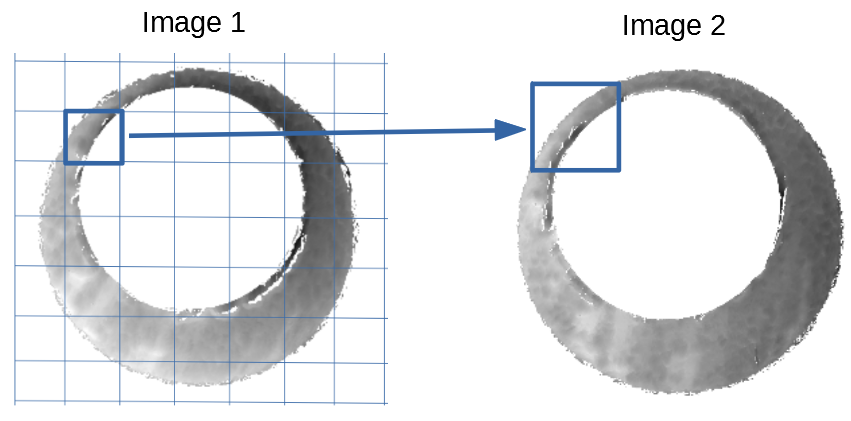
\includegraphics[width=0.5\linewidth]{images/joeZ/im1_im2_cellComparison} 

}

\caption{Comparing a cell in image 1 to a larger region in image 2. We wish to find the translations of the image 1 cell that yield the highest correlation within the image 2 region.}\label{fig:unnamed-chunk-6}
\end{figure}

For the sake of an example, let's focus on the blue outlined cell in image 1. Our goal is to use the image 1 cell to ``search'' a corresponding larger region in image 2 for the horizontal/vertical translations needed to produce the highest correlation. Below is a zoomed-in version of the blue outlined image 1 cell on the left and the larger image 2 region (approximately: I made the gridded image above by-hand outside of R while the images below are from R). The image 1 cell may look larger than the image 2 region, but we can see from the axes that the image 2 region is indeed larger. Any white pixels in the two images are NA values that need to be dealt with in some way before we can use FFTs to calculate the cross-correlation.

\begin{figure}

{\centering 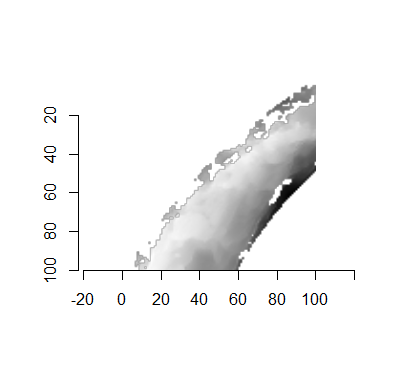
\includegraphics[width=0.5\linewidth]{images/joeZ/im1_split} 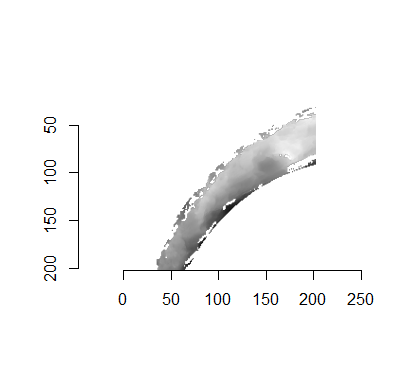
\includegraphics[width=0.5\linewidth]{images/joeZ/im2_split} 

}

\caption{(Left) A cell from image 1. (Right) A region from image 2 centered in the same location as the image 1 cell, yet quadruple the area.}\label{fig:unnamed-chunk-7}
\end{figure}

As already discussed above, one ``solution'' is to replace the NA values with the average pixel value of each image. However, to avoid creating a stronger artificial signal than necessary, we can crop-out the NA rows and columns from the two images above. Below is the cropped version of the two images. The cropping doesn't produce signficantly different images in this case, but you could imagine other examples in which a cell has captured only small amount of breechface in the corner. Such examples are fairly common and cropping signficantly changes the resulting correlation values.

\begin{figure}

{\centering 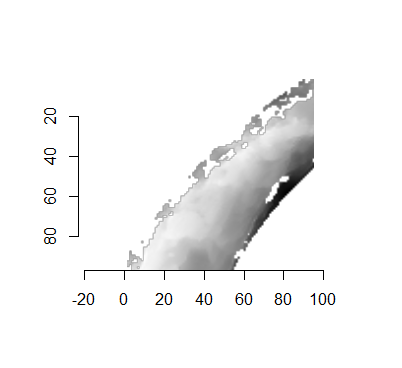
\includegraphics[width=0.5\linewidth]{images/joeZ/im1_splitFilteredCropped} 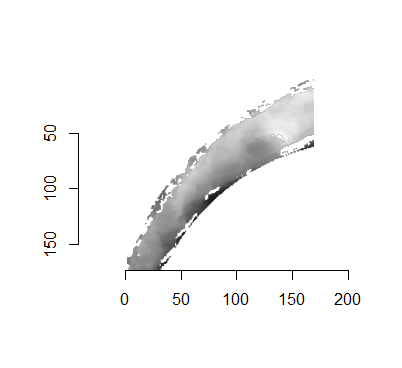
\includegraphics[width=0.5\linewidth]{images/joeZ/im2_splitFilteredCropped} 

}

\caption{The same images as above after cropping NA rows/columns.}\label{fig:unnamed-chunk-8}
\end{figure}

The last step before calculating correlation for these cells is to replace the remaining NAs with the average pixel value. This is shown below.

\begin{figure}

{\centering 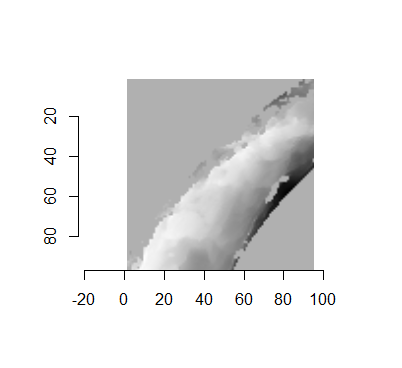
\includegraphics[width=0.5\linewidth]{images/joeZ/im1_splitShifted} 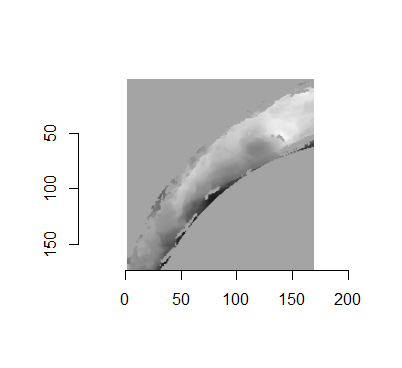
\includegraphics[width=0.5\linewidth]{images/joeZ/im2_splitShifted} 

}

\caption{The NA-cropped images with remaining NAs replaced with the image's average pixel values.}\label{fig:unnamed-chunk-9}
\end{figure}

The cross-correlation is then calculated between these two images via a standard fast fourier transform process (see \href{http://mathworld.wolfram.com/Cross-CorrelationTheorem.html}{Cross-Correlation Theorem}). The benefit of using such a process is that (as the name suggests) it's faster than calculating the raw correlation between the two images. Also, the translations that produce the highest correlation between the image 1 cell and the image 2 region fall out of the calculation for free.

This pre-processing/cross-correlation calculation procedure is repeated for every cell in image 1 that contains breech face. Because it is not valid to assume that the two images are rotationally aligned by default, we perform the same procedure repeatedly while rotating image 2. Currently, we perform a ``rough'' grid search of \(\theta \in [-177.5,180]\) by increments of \(2.5^{\circ}\). Theoretically, the final results tell us how we need to horizontally/vertically translate and rotate the two images to be correctly aligned.

\hypertarget{congruent-matching-tori-a-promising-solution-to-the-missing-value-problem}{%
\subsubsection{Congruent Matching Tori: a promising solution to the missing value problem}\label{congruent-matching-tori-a-promising-solution-to-the-missing-value-problem}}

As discussed above, dealing with missing values is provign to be a pain. The good news is that the currently-implemented CMC as described above yields results very similar to those published in Song et al.~(2015) that originally describes that CMC algorithm. While our results seem to agree with currently published results, it would be nice if we could avoid needing to artifically replace missing values. We can do so if, rather than breaking up the circular breech face scans into disjoint squares, we break up the breech face into donut-shaped regions containing only breech face. Below is an example of such a toroidal region.

\begin{figure}

{\centering 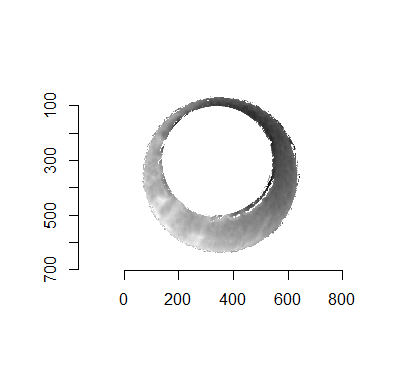
\includegraphics[width=0.5\linewidth]{images/joeZ/im1_original} 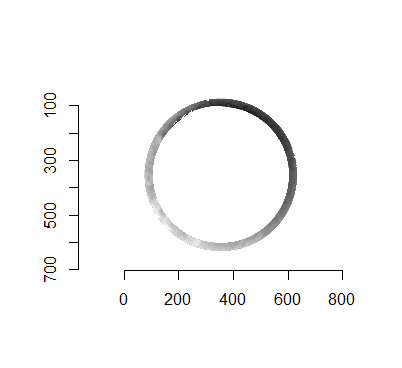
\includegraphics[width=0.5\linewidth]{images/joeZ/im1_toroidalRegion} 

}

\caption{(Left) The original breech face scan image. (Right) A donut-shaped region cut out of the original image.}\label{fig:unnamed-chunk-10}
\end{figure}

By comparing such regions instead of the square cells, we would presumably only need to fill in a few missing value ``holes'' in the breech face scan rather than completely replacing a non-existent signal with an artificial one. In the near-future, I hope to finish up the pre-processing needed for this Congruent Matching Tori method by performing a polar transformation on these images to make them into strips that can easily be compared via an FFT.

\hypertarget{people-involved}{%
\section{People involved}\label{people-involved}}

\hypertarget{faculty}{%
\subsection{Faculty}\label{faculty}}

\begin{itemize}
\tightlist
\item
  Heike Hofmann
\item
  Susan VanderPlas
\end{itemize}

\hypertarget{graduate-students}{%
\subsection{Graduate Students}\label{graduate-students}}

\begin{itemize}
\tightlist
\item
  Ganesh Krishnan
\item
  Kiegan Rice
\item
  Nate Garton
\item
  Charlotte Roigers
\item
  Joe Zemmels
\item
  Yawei Ge
\end{itemize}

\hypertarget{undergraduates}{%
\subsection{Undergraduates}\label{undergraduates}}

\begin{itemize}
\tightlist
\item
  Talen Fisher (fix3p)
\item
  Andrew Maloney
\item
  Mya Fisher, Allison Mark, Connor Hergenreter, Carley McConnell, Anyesha Ray (scanner)
\end{itemize}

\hypertarget{handwriting}{%
\chapter{Handwriting}\label{handwriting}}

We describe our methods for going about the handwriting project here.

\hypertarget{glass}{%
\chapter{Glass}\label{glass}}

\hypertarget{shoes}{%
\chapter{Shoes}\label{shoes}}

\hypertarget{longitudinal}{%
\section{Longitudinal Shoe Study}\label{longitudinal}}

\href{https://github.com/CSAFE-ISU/Longitudinal_Shoe_Study}{Github repository}

\hypertarget{original-study-description}{%
\subsection{Original Study Description}\label{original-study-description}}

\hypertarget{database-paper}{%
\subsection{Database Paper}\label{database-paper}}

\href{https://github.com/CSAFE-ISU/Longitudinal_Shoe_Study/tree/master/Paper}{Paper subdirectory of Github repository}

\hypertarget{methods-and-data-description}{%
\subsubsection{Methods and Data Description}\label{methods-and-data-description}}

Methods and data description handed off to Alicia for editing

\hypertarget{data-analysis-tools}{%
\subsubsection{Data Analysis Tools}\label{data-analysis-tools}}

\begin{itemize}
\tightlist
\item
  Working with the \texttt{EBImage} package - very fast processing of images
\end{itemize}

\hypertarget{film-and-powder-images}{%
\paragraph{Film and Powder Images}\label{film-and-powder-images}}

Analysis Steps:

\begin{enumerate}
\def\labelenumi{\arabic{enumi}.}
\item
  Create threshold mask

  \begin{enumerate}
  \def\labelenumii{\alph{enumii}.}
  \item
    Invert the image\\
  \item
    Blur image (circular/gaussian blur, diameter 5)\\
  \item
    Threshold image (adaptive threshold, 10 x 10 region, keep anything with an average higher than .90 from the mean)\\
  \item
    Expand mask\\
    (default parameters rad1 = 5, rad2 = 91, proportion, expand\_rad = 50)\\

    \begin{enumerate}
    \def\labelenumiii{\arabic{enumiii}.}
    \tightlist
    \item
      erode mask image (circle, diameter rad1)
    \item
      dilate mask image (circle, diameter rad2)
    \item
      label disjoint regions of the image
    \item
      prune small image regions (area \textless{} proportion parameter)
    \item
      set background color
    \item
      create dataframe of useful (non-background) pixels
    \item
      fill in holes and concave regions in mask, then expand by expand\_rad vertically and horizontally (similar to ``convex hull'', but faster and with additional expansion)
    \end{enumerate}
  \end{enumerate}
\item
  Mask image to remove extra variability unrelated to the shoe\\
\item
  Threshold masked image?\\
\end{enumerate}

\hypertarget{wear-characterization}{%
\paragraph{Wear Characterization}\label{wear-characterization}}

Ideas:
- average intensity of cleaned image
- length of border/edges detected

\hypertarget{connor}{%
\section{Passive Shoe Recognition}\label{connor}}

\hypertarget{soyoung}{%
\section{Maximum Clique Matching}\label{soyoung}}

\hypertarget{cocoa}{%
\section{Cocoa Powder Citizen Science}\label{cocoa}}

\hypertarget{theoretical-foundations}{%
\chapter{Theoretical foundations}\label{theoretical-foundations}}

\hypertarget{nates-updates-952019}{%
\section{Nate's Updates 9/5/2019}\label{nates-updates-952019}}

\begin{itemize}
\tightlist
\item
  Currently in Virginia
\item
  RA for this semester (year?) is under Danica
\item
  \textbf{Central Goals}:

  \begin{itemize}
  \tightlist
  \item
    continue work started by Danica and Peter Vergeer on the analysis of likelihood ratios
  \item
    study the differences between specific source (SS) and common source (CS) likelihood ratios (LRs) in an information theoretic way
  \item
    does the CS or SS LR have more ``information''?
  \item
    can be the CS or SS hypotheses (prosecution or defense) be formally compared in terms of being easier to ``prove'' or ``disprove''?
  \end{itemize}
\item
  \textbf{Basic Setup}

  \begin{itemize}
  \tightlist
  \item
    \(H_p\), \(H_d\) are CS prosecution and defense hypotheses upon which we will place priors\\
  \item
    \(A\) and \(B\) are discrete r.v.'s representing two ``sources'' of evidence

    \begin{itemize}
    \tightlist
    \item
      distributions for \(A\) and \(B\) defined conditionally based on the hypothesis
    \item
      SS hypothesis is represented by the conditional random variable \(H_p|A\)
    \end{itemize}
  \item
    \(X\) is data coming from \(A\), \(Y\) is data coming from \(B\)
  \item
    compare information contained in \((X,Y)\) about \(H_p\) and \(H_p|A\)

    \begin{itemize}
    \tightlist
    \item
      this is what I'm working on now
    \item
      important quantities:

      \begin{itemize}
      \tightlist
      \item
        Kullback-Leibler divergences, entropy, mutual information
      \end{itemize}
    \end{itemize}
  \end{itemize}
\end{itemize}

\hypertarget{outreach-activities}{%
\chapter{Outreach activities}\label{outreach-activities}}

\bibliography{book.bib,packages.bib}


\end{document}
